%...existing code...
% !TeX root = main-project01.tex
\documentclass[12pt,twoside,a4paper,openany]{report}
% === Put them here, in the preamble ===
\usepackage{afterpage}
% Load project structure if available; don't fail LaTeX if file is missing

\input{../Structure4all.tex}
%font edit
\usepackage{silence}
\usepackage[no-math]{fontspec}     % ← crucial: prevents fontspec from setting math font
\setmainfont{Arial}                % or your exact font name
\usepackage{mathastext}    % load AFTER fontspec + no-math

\input{headerfooter-project01.tex}

%------------------------%
%document DOCUMENT START
%------------------------%

\begin{document}
%cover
%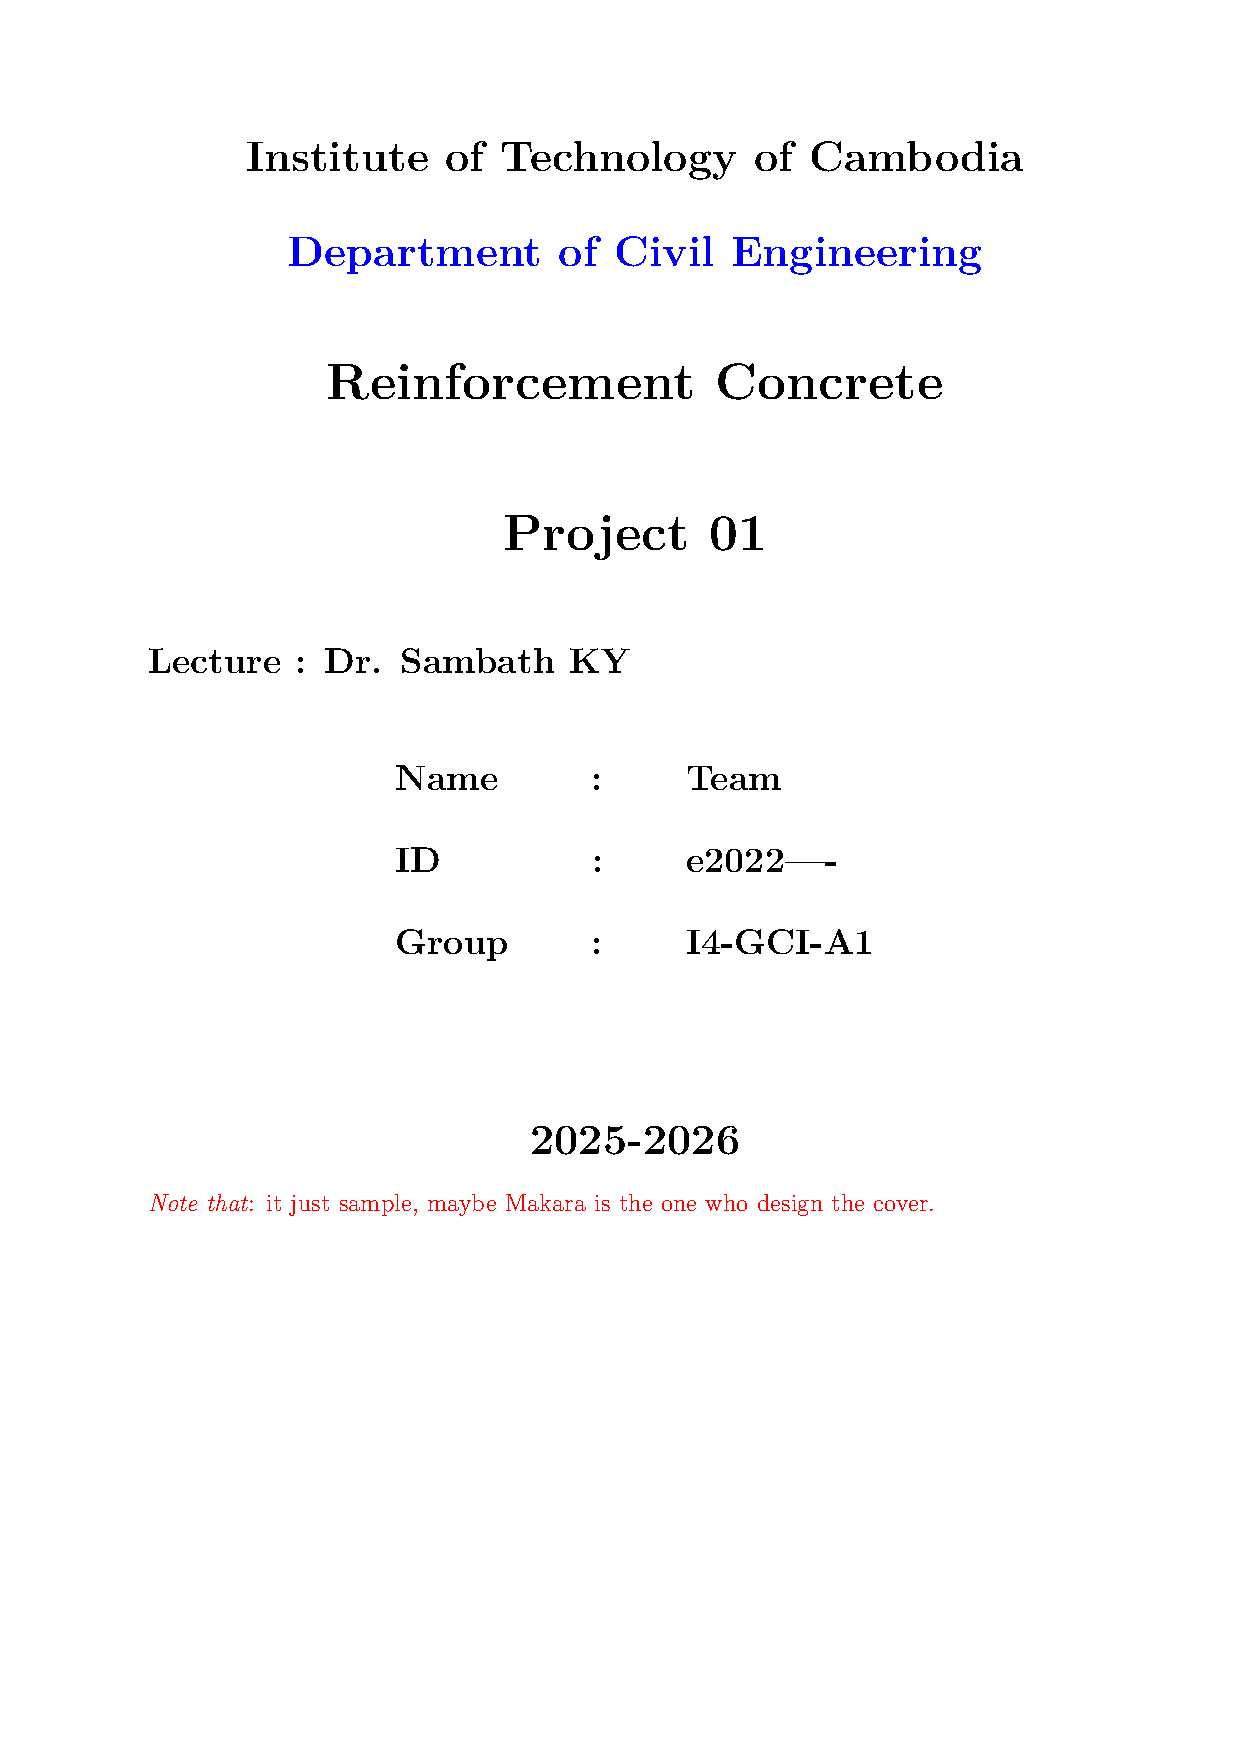
\includepdf[pages=-]{Cover (2)}
% Include substructure file if present; otherwise continue without error
%------------------------%
% Front matter
%------------------------%

\pagestyle{plain} % Default for title page
% Title page
\begin{titlepage}
    \centering
    \vspace*{\fill}
    {\fontsize{30}{30}\selectfont\bfseries \color{blue} RC Design \par \fontsize{60}{60}\selectfont\bfseries \color{blue} Project 01\par}
    \vspace{1cm}
    {\fontsize{20}{50}\selectfont\bfseries \par}
    \vspace*{\fill}
    {\fontsize{16}{16}\selectfont\bfseries \color{red} We can delete this since it no need}
\end{titlepage}
\clearpage
\blankpages{1}
\clearpage
\newgeometry{
  inner=3.5cm,
  outer=2.5cm,
  top=2.5cm,
  bottom=2.5cm
}
\pagenumbering{roman}
\setcounter{page}{1}
%------------------------%
%toc Table of Contents
%------------------------%
\markboth{Contents}{Table of Contents}       % Set header text
\renewcommand{\contentsname}{Table of Contents} %titleoftoc change title of toc
{\fontsize{14}{18}\selectfont\bfseries \color{blue}
\tableofcontents}
\thispagestyle{frontlists}          % Force header on first page
\clearpage

%------------------------%
%lof List of Figures
%------------------------%
\markboth{List of Figures}{List of Figures}
\listoffigures
\thispagestyle{frontlists}          % Force header on first page
\clearpage

%------------------------%
%lot List of Tables
%------------------------%
\markboth{List of Tables}{List of Tables}
\listoftables
\thispagestyle{frontlists}          % Force header on first page
\clearpage
\blankpages{2}
\clearpage

\pagestyle{maincontent}
\pagenumbering{arabic}
\setcounter{page}{1}
%------------------------%
% Main content
%------------------------%

     % Use main content headers
% ------------------------------------------------
%header: VERY IMPORTANT
% Make chapter pages use maincontent style
% ------------------------------------------------
\makeatletter
\let\ps@plain\ps@maincontent
\makeatother
%\renewcommand{\chaptermark}[1]{\markboth{Chapter \thechapter}{#1}}
\renewcommand{\subsectionmark}[1]{\markright{\thesubsection\quad #1}}
\renewcommand{\sectionmark}[1]{\markright{\thesection\quad #1}}


% % Store the current section title whenever \sectionmark is called
% \newcommand{\currentsectiontitle}{}
% \let\oldsectionmark\sectionmark
% \renewcommand{\sectionmark}[1]{%
%   \oldsectionmark{#1}%
%   \renewcommand{\currentsectiontitle}{\thesection\quad #1}%
% }

% % Also store subsection
% \let\oldsubsectionmark\subsectionmark
% \renewcommand{\subsectionmark}[1]{%
%   \oldsubsectionmark{#1}%
%   \renewcommand{\currentsectiontitle}{\thesubsection\quad #1}%
% }

% % Patch longtable to restore the mark on each page
% \makeatletter
% \patchcmd{\LT@output}
%   {\global\advance\c@LT@tables\@ne}
%   {\global\advance\c@LT@tables\@ne
%    \ifx\currentsectiontitle\@empty\else\markright{\currentsectiontitle}\fi}
%   {}{}
% \makeatother
%starttext...... Start texing.....
\clearpage
\newgeometry{
  inner=3.5cm,
  outer=2.5cm,
  top=2.5cm,
  bottom=2.5cm
}
\section{How to Design}
\begin{itemize}
    \item Building Load contains : \textbf{gravity} and \textbf{lateral} Loads.
\end{itemize}
\subsection{Convert Area Loads to Line Load on Beams}
Slabs distribute their load to beam depending on slab span direction and support condition (Eurocode 2, Section on Slabs \cite{EN1992-1-1-2023(1)}; IStructE Manual, Chapter 4 \cite{IStructE2006(6)}).
\subsubsection*{The Tributary Width Method (IStructE Manual, Chapter 4 \cite{IStructE2006(6)}):}
For a \textbf{one-way slab}, load goes to the beams on the short sides:
\begin{center}
\begin{tcolorbox}[colback=white]
Beam Line Load (kN/m) = Floor Load (kN/m2) \(\times\) Tributary Width (m)
\end{tcolorbox}
\end{center}
\textbf{Tributary Width} = half the slab span on each side of the beam (IStructE Manual, Cl. 3.2 \cite{IStructE2006(6)}). \\[2mm]
\textbf{Example}: If Slab spans 5m between two beams, so each beam take \(5/2 = 2.5m\) tribuyary width. And if floor load is 10kN/m2, then beam line load is \( 10 \times 2.5 = 25 kN/m\) \\[2mm]
For a \textbf{two-way slab}, load distributes in both directions
(Eurocode 2, Section on Two-Way Slabs \cite{EN1992-1-1-2023(1)}; IStructE Manual, Chapter 5 \cite{IStructE2006(6)}):
\begin{itemize}
    \item Short span beam take triangular load
    \item Long span beam take trapezoidal load
\end{itemize}
\subsection{Apply ULS and SLS Load Combinations}
\begin{itemize}
    \item ULS (Ultimate Limit State) - for stength design
    \[\sum_{i} \gamma_{G,i} G_{k,i} + \gamma_{Q,1} Q_{k,1} + \sum_{j>1} \gamma_{Q,j} \varphi_{0.j} Q_{k,j}\]
    \item SLS (serviceability Limit State) - for deflection/crack check \\[2mm]
    Chearacteristic Combinations: \[\sum_{i}G_{k,i} + Q_{k,1} + \sum_{j>1} \varphi_{0,j} Q_{k,j} + (P_k)\]
    Quasi-permanent (for long-term deflection)
    \[\sum_{i}G_{k,i} + \sum_{j}\varphi_{2,j} Q_{k,j} + (P_k)\]
\end{itemize}
\subsection{Beam Support Conditions}
Support conditions determine the bending moment diagram shape and therefore where reinforcement must be placed
(Eurocode 2, Section on Structural Analysis \cite{EN1992-1-1-2023(1)}; IStructE Manual, Chapter 4 \cite{IStructE2006(6)}):
\begin{table}[H]
\centering
\caption{Beam support condition}
\resizebox{\linewidth}{!}{
\begin{tabular}{LLL}
\toprule
\textbf{Support Type}     & \textbf{Description}          & \textbf{Moment at Support} \\\midrule
\textbf{Simply supported} & Beam sits on wall/pad         & Zero moment at ends        \\
\textbf{Continuous beam}  & Multiple spans, monolithic    & Hogging moment at supports \\
\textbf{Fixed end}        & Fully restrained (rare in RC) & Full fixity moment         \\
\textbf{Partially fixed}  & Column/beam junction          & Partial moment transfer \\ \bottomrule
\end{tabular}}
\end{table}
\begin{table}[H]
\centering
\resizebox{\linewidth}{!}{
\begin{tabular}{LLLL}
\textbf{Support Type} & \textbf{Rotation Allowed} & \textbf{Moment at Support} & \textbf{Typical Structure} \\
Simply Supported      & Yes                       & 0                          & Beam on columns            \\
Continuous            & Small rotation            & Negative moment            & Multi-span floor beam      \\
Fixed                 & No rotation               & Maximum moment             & Cantilever                 \\
Partially Fixed       & Limited rotation          & Partial moment             & Beam-column joint
\end{tabular}}
\end{table}
\noindent In reinforced concrete buildings, beams are almost always continuous over columns because they are cast monolithically
(IStructE Manual, Chapter 4, Cl. 4.2 \cite{IStructE2006(6)}).
\subsection{Design Workflow}
\begin{itemize}
  \item \textbf{STEP 1:} Establish building layout and use

  \item \textbf{STEP 2:} Identify slab type (one-way / two-way)

  \item \textbf{STEP 3:} Gather \(G_k\), permanent loads \\
  (EN 1991-1-1:2002, Annex A, Table A.1 \cite{EN1991-1-1-2002(3)})

  \item \textbf{STEP 4:} Gather \(Q_k\), variable loads \\
  (EN 1991-1-1:2002, Cl. 6.3.1, Table 6.2 \cite{EN1991-1-1-2002(3)})

  \item \textbf{STEP 5:} Apply ULS combination

  \item \textbf{STEP 6:} Convert to beam line load

  \item \textbf{STEP 7:} Calculate bending moments and shear \\
  (IStructE Manual, Ch. 4 \cite{IStructE2006(6)}) \\
  (Eurocode 2, Structural Analysis \cite{EN1992-1-1-2023(1)})

  \item \textbf{STEP 8:} Size beam using \(L/d\) ratio \\
  (Eurocode 2, Deflection Section \cite{EN1992-1-1-2023(1)})

  \item \textbf{STEP 9:} Design reinforcement \\
  (Eurocode 2, ULS Design Section \cite{EN1992-1-1-2023(1)})

  \item \textbf{STEP 10:} Check SLS — deflection and cracking \\
  (EN 1990:2002, Cl. 6.5 \cite{EN1990-2002(5)}) \\
  (Eurocode 2, SLS Section \cite{EN1992-1-1-2023(1)})

  \item \textbf{STEP 11:} Detail and produce drawings \\
  (Eurocode 2, Detailing Section \cite{EN1992-1-1-2023(1)}) \\
  (IStructE Manual, Ch. 4 \cite{IStructE2006(6)})
\end{itemize}
\subsection{The Key Distinction: what are we Designing}
According to
(IStructE Manual, Chapter 3 \cite{IStructE2006(6)}):
\begin{table}[H]
\centering
\begin{tabular}{LL}
\toprule
\textbf{Element} & \textbf{How Load Works}               \\\midrule
Beam             & Carries only load from its own floor  \\
Column           & Carries load from all floors above it \\
Foundation       & Carries load from the entire building \\ \bottomrule
\end{tabular}
\caption{How structure work}
\end{table}
\subsection{The Unit Journey}
\begin{table}[H]
\resizebox{\linewidth}{!}{
\begin{tabular}{LLLL}
\toprule
\textbf{Unit} & \textbf{Name} & \textbf{Used For}        & \textbf{How We Get It}    \\ \midrule
kN/m³         & Density       & Material property        & Given in \cite{EN1991-1-1-2002(3)} Table A.1 \\
kN/m²         & Area load     & Slab design              & Density \(\times\) thickness        \\
kN/m          & Line load     & Beam design              & kN/m² \(\times\) tributary width    \\
kN            & Point force   & Column/foundation design & kN/m \(\times\) span \(\div\) 2            \\ \bottomrule
\end{tabular}}
\caption{Unit of load to consider in design}
\end{table}
\clearpage
\section{Introduction}
hello \( y = ax + b = 2 + 3\)
This is Our Team Intro.

\clearpage
\section{Detailed Design Calculations}
\subsection{Load}
For imposed laods on floor according to Table $6.1 - 6.4$ in EN 1991-1-1:2002 \cite{EN1991-1-1-2002(3)}. Is summary in Table \ref{tab:imposedload}.
% Please add the following required packages to your document preamble:

\begin{longtable}{|L|L|C|C|}
\caption{Imposed Loads On Floor Base On EN 1991-1-1:2002} \label{tab:imposedload} \\
\hline
\multicolumn{1}{|C|}{\textbf{Category}} & \multicolumn{1}{C|}{\textbf{Sub-category / Use}}                                                                                 & \textbf{\begin{tabular}[C]{@{}C@{}}$q_k$ \\ {[}kN/m²{]}\end{tabular}} & \textbf{\begin{tabular}[C]{@{}C@{}}$Q_k$\\  {[}kN{]}\end{tabular}} \\ \hline
\endfirsthead
\multicolumn{4}{c}{{\tablename\ \thetable{:} Imposed Loads On Floor Base On EN 1991-1-1:2002}} \\[2mm]
\hline
\multicolumn{1}{|C|}{\textbf{Category}} & \multicolumn{1}{C|}{\textbf{Sub-category / Use}}                                                                                 & \textbf{\begin{tabular}[C]{@{}C@{}}$q_k$ \\ {[}kN/m²{]}\end{tabular}} & \textbf{\begin{tabular}[C]{@{}C@{}}$Q_k$\\  {[}kN{]}\end{tabular}} \\ \hline
\endhead
\multicolumn{4}{r}{{Continued on next page}} \\
\endfoot
\endlastfoot

\multirow{4}{*}{\textbf{Category A}}    & \begin{tabular}[C]{@{}L@{}}Areas for domestic and \\ residential activities\end{tabular}                                         &                                                                      &                                                                   \\ \cline{2-4}
                                        & - Floors                                                                                                                         & 1,5 to 2,0                                                           & 2,0 to 3,0                                                        \\ \cline{2-4}
                                        & - Stairs                                                                                                                         & 2,0 to 4,0                                                           & 2,0 to 4,0                                                        \\ \cline{2-4}
                                        & - Balconies                                                                                                                      & 2,5 to 4,0                                                           & 2,0 to 3,0                                                        \\ \hline
\textbf{Category B}                     & Office areas                                                                                                                     & 2,0 to 3,0                                                           & 1,5 to 4,5                                                        \\ \hline
\textbf{Category C}                     & \begin{tabular}[C]{@{}L@{}}Areas where people \\ may congregate\end{tabular}                                                     &                                                                      &                                                                   \\ \hline
C1                                      & \begin{tabular}[C]{@{}L@{}}Areas with tables \\ (e.g. schools, cafes,\\  restaurants, \\ reading rooms)\end{tabular}             & 2,0 to 3,0                                                           & 3,0 to 4,0                                                        \\ \hline
C2                                      & \begin{tabular}[C]{@{}L@{}}Areas with fixed seats \\ (e.g. theatres,\\  cinemas,\\  churches)\end{tabular}                       & 3,0 to 4,0                                                           & \begin{tabular}[C]{@{}C@{}}2,5 to 7,0 \\ (4,0)\end{tabular}       \\ \hline
C3                                      & \begin{tabular}[C]{@{}L@{}}Areas without obstacles\\ for moving people\\ (e.g. museums, \\ entrance halls)\end{tabular}          & 3,0 to 5,0                                                           & 4,0 to 7,0                                                        \\ \hline
C4                                      & \begin{tabular}[C]{@{}L@{}}Areas with possible physical\\ activities \\ (e.g. dance halls, gyms)\end{tabular}                    & 3,5 to 5,0                                                           & 3,5 to 7,0                                                        \\ \hline
C5                                      & \begin{tabular}[C]{@{}L@{}}Areas susceptible to \\ large crowds\\ (e.g. concert halls, \\ sports halls with stands)\end{tabular} & 5,0 to 7,5                                                           & 3,5 to 4,5                                                        \\ \hline
\textbf{Category D}                     & Shopping areas                                                                                                                   &                                                                      &                                                                   \\ \hline
D1                                      & Areas in general retail shops                                                                                                    & 4,0 to 5,0                                                           & \begin{tabular}[C]{@{}C@{}}3,5 to 7,0 \\ (4,0)\end{tabular}       \\ \hline
D2                                      & Areas in department stores                                                                                                       & 4,0 to 5,0                                                           & 3,5 to 7,0                                                        \\ \hline
\textbf{Category E}                     & \begin{tabular}[C]{@{}L@{}}Storage and industrial\\ activities\\ (general storage,\\  accessible areas)\end{tabular}             & 7,5                                                                  & 7,0                                                               \\ \hline
\end{longtable}
\vspace*{2em}
\noindent And this is the imposed loads on second floor that we assumed. which shown in Table \ref{tab:imposedloadsecondfl}.
\begin{longtable}{|C|L|C|C|}
\caption{Imposed Loads On Second Floor} \label{tab:imposedloadsecondfl}\\
\hline
\textbf{No.} & \multicolumn{1}{c|}{\textbf{Room / Area}}                                   & \textbf{\begin{tabular}[C]{@{}C@{}}Category\\ (EN 1991-1-1)\end{tabular}} & \textbf{\begin{tabular}[C]{@{}C@{}}$q_k$\\  (kN/m2)\end{tabular}} \\ \hline
\endfirsthead
\multicolumn{4}{C}{\tablename\ \thetable{:} Imposed Loads On Second Floor} \\[2mm]
\hline
\textbf{No.} & \multicolumn{1}{c|}{\textbf{Room / Area}}                                   & \textbf{\begin{tabular}[C]{@{}C@{}}Category\\ (EN 1991-1-1)\end{tabular}} & \textbf{\begin{tabular}[C]{@{}C@{}}$q_k$\\  (kN/m2)\end{tabular}} \\ \hline
\endhead
\multicolumn{4}{r}{Continued on next page} \\
\endfoot
\endlastfoot
1            & \begin{tabular}[C]{@{}L@{}}Receptionist/\\  Reception\end{tabular}          & B                                                                         & 3                                                                \\ \hline
2            & \begin{tabular}[C]{@{}L@{}}Workstation /\\ Open office\end{tabular}         & B                                                                         & 3                                                                \\ \hline
3            & Meeting   Room                                                              & C1                                                                        & 3                                                                \\ \hline
4            & President   Office                                                          & B                                                                         & 3                                                                \\ \hline
5            & Vice   President Offices                                                    & B                                                                         & 3                                                                \\ \hline
6            & Accounting                                                                  & B                                                                         & 3                                                                \\ \hline
7            & \begin{tabular}[C]{@{}L@{}}General   Sale \&\\  Administration\end{tabular} & B                                                                         & 3                                                                \\ \hline
8            & \begin{tabular}[C]{@{}L@{}}Copy   / \\ Printer Area\end{tabular}            & B                                                                         & 3                                                                \\ \hline
9            & Storages                                                                    & E1                                                                        & 5                                                                \\ \hline
10           & \begin{tabular}[C]{@{}L@{}}Lift   Lobby /\\ Lift Area\end{tabular}          & C3                                                                        & 4                                                                \\ \hline
11           & Stair   (Main Stair)                                                        & A                                                                         & 4                                                                \\ \hline
12           & Restroom   (Men)                                                            & B                                                                         & 3                                                                \\ \hline
13           & Restroom   (Women)                                                          & B                                                                         & 3                                                                \\ \hline
14           & \multicolumn{1}{c|}{—}                                                      & —                                                                         & —                                                                \\ \hline
15           & \multicolumn{1}{c|}{—}                                                      & —                                                                         & —                                                                \\ \hline
16           & \multicolumn{1}{c|}{—}                                                      & —                                                                         & —                                                                \\ \hline
17           & Entrance                                                                    & C3                                                                        & 4                                                                \\ \hline
18           & Emergency Stair                                                             & A                                                                         & 4                                                                \\ \hline
19           & \begin{tabular}[C]{@{}L@{}}Server\&\\ Technical Room\end{tabular}           & \begin{tabular}[C]{@{}C@{}}E1  \\  (conservative)\end{tabular}            & 5                                                                \\ \hline
20           & \begin{tabular}[C]{@{}L@{}}Kitchen /\\ Pantry\end{tabular}                  & C1                                                                        & 3                                                                \\ \hline
21           & Library                                                                     & C3                                                                        & 4                                                                \\ \hline
22           & Share Space                                                                 & C3                                                                        & 4                                                                \\ \hline
\end{longtable}







\clearpage
%referennces
\markboth{References}{References}   % set mark BEFORE the page
\phantomsection %Creates a hyperlink anchor (jump to that page when click)
\renewcommand{\chapter}{\section}
\renewcommand{\thechapter}{} % edit chapter numbering from here.
\renewcommand{\bibname}{References}  % change Bibliography -> References globally
%\thispagestyle{empty}  % optional: remove headers/footers

\begin{thebibliography}{99}
\addcontentsline{toc}{section}{References}

\bibitem{EN1992-1-1-2023(1)}
BSI, \textit{BS EN 1992-1-1:2023 - Eurocode 2:
Design of concrete structures - Part 1-1:
General rules and rules for buildings, bridges
and civil engineering structures},
BSI Standards Publication, 2023.

\bibitem{EN1991-1-1-2025(2)}
BSI, \textit{BS EN 1991-1-1:2025 - Eurocode 1:
Actions on structures - Part 1-1: Specific weight
of materials, self-weight of construction works
and imposed loads for buildings},
BSI Standards Publication, 2025.

\bibitem{EN1991-1-1-2002(3)}
CEN, \textit{EN 1991-1-1:2002 - Eurocode 1:
Actions on structures - Part 1-1: General actions
- Densities, self-weight, imposed loads for
buildings}, European Committee for
Standardization, 2002.
[Online]. Available:
\url{https://www.phd.eng.br/wp-content/uploads/
2015/12/en.1991.1.1.2002.pdf}

\bibitem{EN1991-1-4-2005(4)}
CEN, \textit{EN 1991-1-4:2005+A1 - Eurocode 1:
Actions on structures - Part 1-4: General actions
- Wind actions}, European Standard, Incorporating
corrigendum January 2010, April 2010.

\bibitem{EN1990-2002(5)}
CEN, \textit{EN 1990:2002 - Eurocode:
Basis of Structural Design},
European Committee for Standardization, 2002.
[Online]. Available:
\url{https://www.phd.eng.br/wp-content/uploads/
2015/12/en.1990.2002.pdf}

\bibitem{IStructE2006(6)}
Institution of Structural Engineers (IStructE),
\textit{Manual for the Design of Concrete Building
Structures to Eurocode 2},
2nd ed., IStructE, London, 2006.
[Online]. Available:
\url{https://archive.org/details/manual-for-the-design-of-concrete-building-
structures-to-eurocode-2}

\end{thebibliography}

\noindent \textcolor{red}{\textit{Note that :} We may use the referennces provide by professor (check in telegram group) if it still not enought we can add more maybe.}

\clearpage
\phantomsection %Creates a hyperlink anchor (jump to that page when click)
\section*{Appendices}
\markboth{Appendices}{Appendices}

%\markright{Appendices} % still make markright work eventhough using \section*{}
\addcontentsline{toc}{section}{Appendices}

% Make sure you have \usepackage{caption} in Structure4all.te
\end{document}
%...existing code...
